\documentclass[pe1a]{tnreport} % If you are in 1nd year
\boolfalse{fise}
\booltrue{fisa}
\usepackage{url}
\usepackage{float}
\usepackage[automake]{glossaries-extra}
\usepackage{tikz}
\usetikzlibrary{shapes.geometric}

%\documentclass[stage1a,confidential]{tnreport} % If you are writing confidential report

\def\reportTitle{Projet d'entreprise de première année} % Titre du mémoire
\def\reportLongTitle{Projet d'entreprise de première année} % Titre plus long du mémoire

\def\reportAuthor{Joris BEGEL}
\def\reportAuthorEmail{\email{joris.begel@telecomnancy.eu}} % Courriel de l'élève

\def\reportAuthorAddress{174 b, rue Charles de Gaulle} % Adresse de l'élève
\def\reportAuthorCity{57290, SEREMANGE-ERZANGE} % Adresse (cont.) de l'élève
\def\reportAuthorPhone{+33 (0)6 03 29 34 73} % Téléphone de l'élève

\def\reportSupervisor{Dominique Budano} % Prénom Nom de l'encadrant industriel
\def\reportAcademicSupervisor{Hervé Panetto} % Prénom Nom de l'encadrant académique

\def\reportCompany{Viessmann} % Nom de l'entreprise d'accueil
\def\reportCompanyAddress{Avenue André Gouy}  % Adresse de l'entreprise
\def\reportCompanyCity{57380, FAULQUEMONT} % Adresse (cont.) de l'entreprise
\def\reportCompanyPhone{+33 (0)3 87 29 17 00} % Téléphone de l'entreprise
\def\reportCompanyLogoPath{figures/test_200} % Logo de l'entreprise -- comment this definition to remove company logo

\def\place{Nancy} % Ville pour la signature pour l'engagement anti-plagiat
\def\date{\today} % Date pour la signature de l'engagement anti-plagiat

% \newacronym{Andon}{Andon}{Système de signalisation visuelle sur les lignes de production}
% \newacronym{IE}{IE}{Industrial Engineer}

\newglossaryentry{WebSocket}{
    name={WebSocket},
    description={Protocole de communication bidirectionnelle persistante entre
    un client et un serveur, permettant au serveur de pousser des messages
    vers le client sans nouvelle requête}
}

\newglossaryentry{Quasar}{
    name={Quasar},
    description={Framework front-end basé sur Vue.js, fournissant un ensemble
    de composants d'interface prêts à l'emploi}
}

\newglossaryentry{Sequelize}{
    name={Sequelize},
    description={ORM (\textit{Object-Relational Mapping}) pour Node.js,
    permettant d'interagir avec une base de données relationnelle via des
    objets JavaScript plutôt qu'en écrivant des requêtes SQL brutes}
}

\newglossaryentry{andons}{
    name={Andons},
    description={Système de signalisation visuelle utilisé sur les lignes de
    production pour communiquer en temps réel l'état d'avancement ou les
    incidents}
}

\newglossaryentry{cron}{
    name={Cron},
    description={Système d'ordonnancement de tâches récurrentes selon une
    syntaxe horaire spécifique}
}

\newglossaryentry{IE}{
    name={IE},
    description={Industrial Engineer}
}

\makeglossaries

\begin{document}

\maketitle
\pagenumbering{roman}

\insertAntiPlagiarismAgreement{BEGEL, Joris}{32211304}

\cleardoublepage

\makesecondtitle

\cleardoublepage

\renewcommand{\baselinestretch}{0.5}\normalsize
\tableofcontents
\renewcommand{\baselinestretch}{1.0}\normalsize
\cleardoublepage

\pagenumbering{arabic}
\setcounter{page}{1}

\chapter{Introduction}

Dans le cadre de ma formation d'ingénieur en informatique, je réalise mon apprentissage au sein de l'entreprise Viessmann, 
dans le Département Digitalisation. Cette expérience me permet de mettre en pratique les connaissances 
acquises à l'école tout en découvrant le fonctionnement d'une entreprise industrielle 
et ses enjeux liés à la transformation numérique.

Le Département Digitalisation accompagne les différents services de l'entreprise dans 
la modernisation de leurs processus, à travers le développement de solutions 
informatiques, l'automatisation des tâches et la gestion des données. En tant 
qu'assistant ingénieur, je participe à des projets concrets ayant un impact direct 
sur l'efficacité des outils internes.

Ce rapport clôture ma première année d'apprentissage et fait suite au rapport 
intermédiaire, dans lequel l'entreprise et son organisation ont été présentées en 
détail. Ce rapport a pour but de rendre compte le travail réalisé sur l'ensemble de 
l'année et des apports de cette expérience. Après un rappel du cadre de travail 
et des missions confiées, deux missions significatives seront détaillées. 
Un bilan des compétences acquises et une analyse permettront ensuite 
de prendre du recul sur cette année, avant d'évoquer les perspectives pour la 
deuxième année d'apprentissage.
\cleardoublepage

% \chapter{Présentation de l'entreprise}

% Fondé en 1917 en tant que fabricant de techniques de chauffage, Viessmann est aujourd'hui l'un des principaux fournisseurs mondiaux de solutions efficaces en matière de climat (chauffage, eau et qualité de l'air) et d'énergies renouvelables pour les secteurs résidentiels et commerciaux.
% L'histoire de Viessmann France débute en 1965 par la création d'une agence à Metz. En 1971, une usine est construite en Moselle, dans la commune de Faulquemont et 130 salariés débutent la production de produits sur une surface couverte de 12 000 m².
% Viessmann fait partie de Carrier Global Corporation, leader mondial des solutions climatiques et énergétiques intelligentes.~\cite{GOT3}

% \begin{table}
% \centering
% \begin{tabular}{|p{4cm}|p{13cm}|}
% \hline
% \textbf{Caractéristiques} & \textbf{Définition / Description} \\
% \hline

% \textbf{Type d’organisation} &
% \begin{itemize}
%     \item Entreprise privée à but lucratif spécialisée dans les solutions de chauffage, de climatisation et de gestion intelligente de l’énergie
%     \item Groupe industriel international fondé en 1917 en Allemagne (Allendorf)
%     \item Appartient au groupe \textbf{Carrier Global Corporation}
%     \item Organisation structurée autour de pôles industriels, commerciaux et de recherche et développement
% \end{itemize} \\
% \hline

% \textbf{Finalité = raison d’être} &
% \begin{itemize}
%  \item \textbf{Economique} : concevoir, produire et commercialiser des solutions énergétiques performantes et innovantes afin d’assurer la croissance, la rentabilité et la pérennité du groupe sur le marché mondial de l’énergie.
%  \item \textbf{Sociale} : garantir de bonnes conditions de travail, favoriser la formation continue, le développement des compétences et l’épanouissement professionnel des salariés, tout en promouvant la qualité de vie au travail.
%  \item \textbf{Sociétale} : contribuer à la transition énergétique et à la protection de l’environnement en développant des technologies durables, en réduisant l’empreinte carbone et en agissant de manière responsable vis-à-vis de la société et des parties prenantes.
% \end{itemize}
% \\
% \hline

% \textbf{Nature de l’activité et but} &
% Fabrication de techniques de chauffage et de gestion de l'énergie.

% Industrie de la technologie énergétique
% \end

% \begin{itemize}
%   \item But lucratif, visant la création de valeur économique par la commercialisation de technologies énergétiques innovantes.
% \end{itemize} \\


% %  \item \textbf{le but lucratif} consiste à rechercher le profit ; c’est le cas des entreprises privées
% % (ex. : Apple, qui cherche à réaliser des bénéfices) ;
% %  \item \textbf{le but non lucratif} consiste à viser un but autre que le profit : partager un loisir (association sportive) ; jouer un rôle humanitaire (ex. : Médecins du Monde), satisfaire l’intérêt général (ex. : éducation) ; c’est le cas des associations et des organisations publiques.
% \hline

% \textbf{Statut juridique} &
% \begin{itemize}
%  \item SAS
% \end{itemize} \\
% \hline

% \textbf{Ressources
% Présentation au niveau France} &
% \begin{itemize}
%  \item Humaines (Collaborateurs qualifiés, expertise technique)
%  \item Financières (Fond d'investissement, capital détenu par actionnaires)
%  \item Matérielles (Usines de production, équipements techniques)
%  \item Immatérielles (Notoritété, brevets, marque déposées)
% \end{itemize} \\
% \hline

% \textbf{Champ d’action géographique} &
% \begin{itemize}
% \item Europe, Amérique du Nord, Asie
% \end{itemize} \\
% \hline

% \textbf{Taille} &
% \begin{itemize}
% \item ETI (500-999 salariés)
% \end{itemize} \\
% \hline

% \textbf{Nationalité} & Allemagne \\

% \hline
% \end{tabular}
% \caption{Fiche de présentation de Viessmann}\label{tab:fiche}
% \end{table}


\cleardoublepage
\chapter{Cadre de travail et missions confiées}

Cette première partie revient brièvement sur le cadre de mon apprentissage et 
met en perspective l'évolution de mon poste depuis le rapport intermédiaire. 
La présentation détaillée de l'entreprise et du service ayant déjà été 
effectuée dans le rapport intermédiaire, je me concentre ici sur les éléments qui ont 
évolué au cours de la seconde moitié de l'année.

\section{Rappel synthétique du périmètre initial}

J'exerce en tant qu'assistant ingénieur au sein du Département Digitalisation 
de Viessmann. Ce service intervient en support des différents métiers de 
l'entreprise pour concevoir, développer et maintenir des outils internes 
visant à moderniser les processus, automatiser les tâches répétitives et 
faciliter la circulation de l'information.

Au cours du semestre 5, période couverte par le rapport intermédiaire, mon 
périmètre portait principalement sur l'application de gestion des 
\textbf{Edge Devices} : des machines installées directement sur les lignes 
de production, dont cette application permet le suivi et la configuration. 
Mes développements sur cet outil étaient réalisés avec le framework 
\textbf{Nuxt}.

Ce premier semestre m'a permis de me familiariser avec l'environnement de 
travail du Département Digitalisation, ses méthodes et son écosystème 
technique, et de réaliser mes premières contributions concrètes sur une 
application réellement exploitée en production.

\section{Évolutions du poste, du service et des missions depuis le rapport intermédiaire}

L'évolution la plus visible depuis le rapport intermédiaire est le changement 
de périmètre applicatif. Au second semestre, je suis passé de l'application 
Edge Devices à l'application \textbf{Shopfloor}, un outil métier utilisé 
quotidiennement par les équipes de production, opérateurs, \textit{team 
leaders} et responsables de secteur. S'agissant d'une application plus
ancienne, sa stack technique diffère de celle des Edge Devices :
je suis passé du framework Nuxt à un développement en \textbf{Express} côté
serveur et \textbf{\gls{Quasar}} côté client. La persistance des données est
gérée via \textbf{\gls{Sequelize}}, un ORM Node.js qui abstrait les requêtes
SQL et facilite la manipulation des modèles de données en JavaScript.

Une particularité de l'écosystème du département est le recours à des
packages npm internes, développés et maintenus par l'équipe elle-même.
Ces packages encapsulent du code partagé entre plusieurs applications :
les \textbf{modèles \gls{Sequelize}} communs (définitions des tables, associations)
ainsi que des modules de \textbf{gestion des credentials} d'accès aux services
internes. Plutôt que de dupliquer ce code dans chaque projet, le département
les publie sous forme de packages versionnés sur un registre interne,
et chaque application déclare ses dépendances de façon explicite. Cette
approche garantit la cohérence des modèles de données entre les différentes
applications et simplifie la mise à jour centralisée des configurations
d'authentification.

Au-delà du changement d'application, mon poste a évolué dans le sens d'une 
autonomie progressivement accrue. Là où mes premières contributions 
consistaient principalement à implémenter des fonctionnalités déjà 
spécifiées, je suis désormais davantage impliqué dans la conception
des fonctionnalités elles-mêmes comme l'analyse du besoin, les choix techniques ou
la modélisation des données.

La nature des tâches confiées a également gagné en envergure. Les missions 
sont passées de développements ponctuels à des fonctionnalités plus 
structurantes, embarquant plusieurs écrans, des règles métier élaborées et 
parfois des mécanismes d'automatisation. La mission de gestion des lignes 
de production, détaillée plus loin, illustre cette montée en envergure.

\section{Nouveaux outils, nouvelles responsabilités}

Plusieurs technologies et librairies se sont ajoutées à mon environnement de 
travail : le protocole \gls{WebSocket} pour la communication temps réel et 
la librairie node-schedule pour la planification de tâches 
automatisées.

Un changement plus structurant est par ailleurs intervenu à l'échelle de 
toute l'entreprise. À la suite du rachat de Viessmann par le groupe américain 
\textbf{Carrier}, l'ensemble du système d'information a dû être migré de 
l'écosystème Google vers l'écosystème Microsoft. Cette 
migration a modifié les outils du quotidien et explique notamment l'adoption 
de SharePoint, désormais utilisé pour la diffusion de la 
documentation à destination des utilisateurs.

Enfin, je suis désormais responsable du début à la fin lors du développement d'une nouvelle fonctionnalité, depuis la
modélisation des données jusqu'à la mise en production et la rédaction de la
documentation utilisateur. Cette responsabilité élargie m'a confronté à des
questions que je ne rencontrais pas auparavant : comment documenter pour un
public non technique, comment garantir la fiabilité d'une fonctionnalité en
production, comment gérer les retours d'utilisateurs après déploiement.

La migration vers l'écosystème Microsoft a également profondément modifié
les modes de communication au quotidien. Les réunions, auparavant organisées
via Google Meet, se tiennent désormais exclusivement sur Microsoft Teams.
Trois types de réunions rythment régulièrement mon activité :

\begin{itemize}
    \item Les réunions IT, auxquelles je participe en tant que membre
    du Département Digitalisation, permettent de coordonner les projets
    transverses, de traiter les problèmes techniques et d'assurer une cohérence
    entre l'équipe digitalisation et l'équipe IT
    \item Les réunions de service, organisées à l'échelle du département,
    servent à synchroniser l'ensemble des collaborateurs sur l'avancement des
    missions, les priorités et les décisions à prendre
    \item Les points réguliers avec mon maître d'apprentissage, plus
    informels, permettent de faire le bilan de mes avancées, d'ajuster les
    priorités et de préparer les prochaines étapes.
\end{itemize}

\begin{figure}[H]
    \centering
    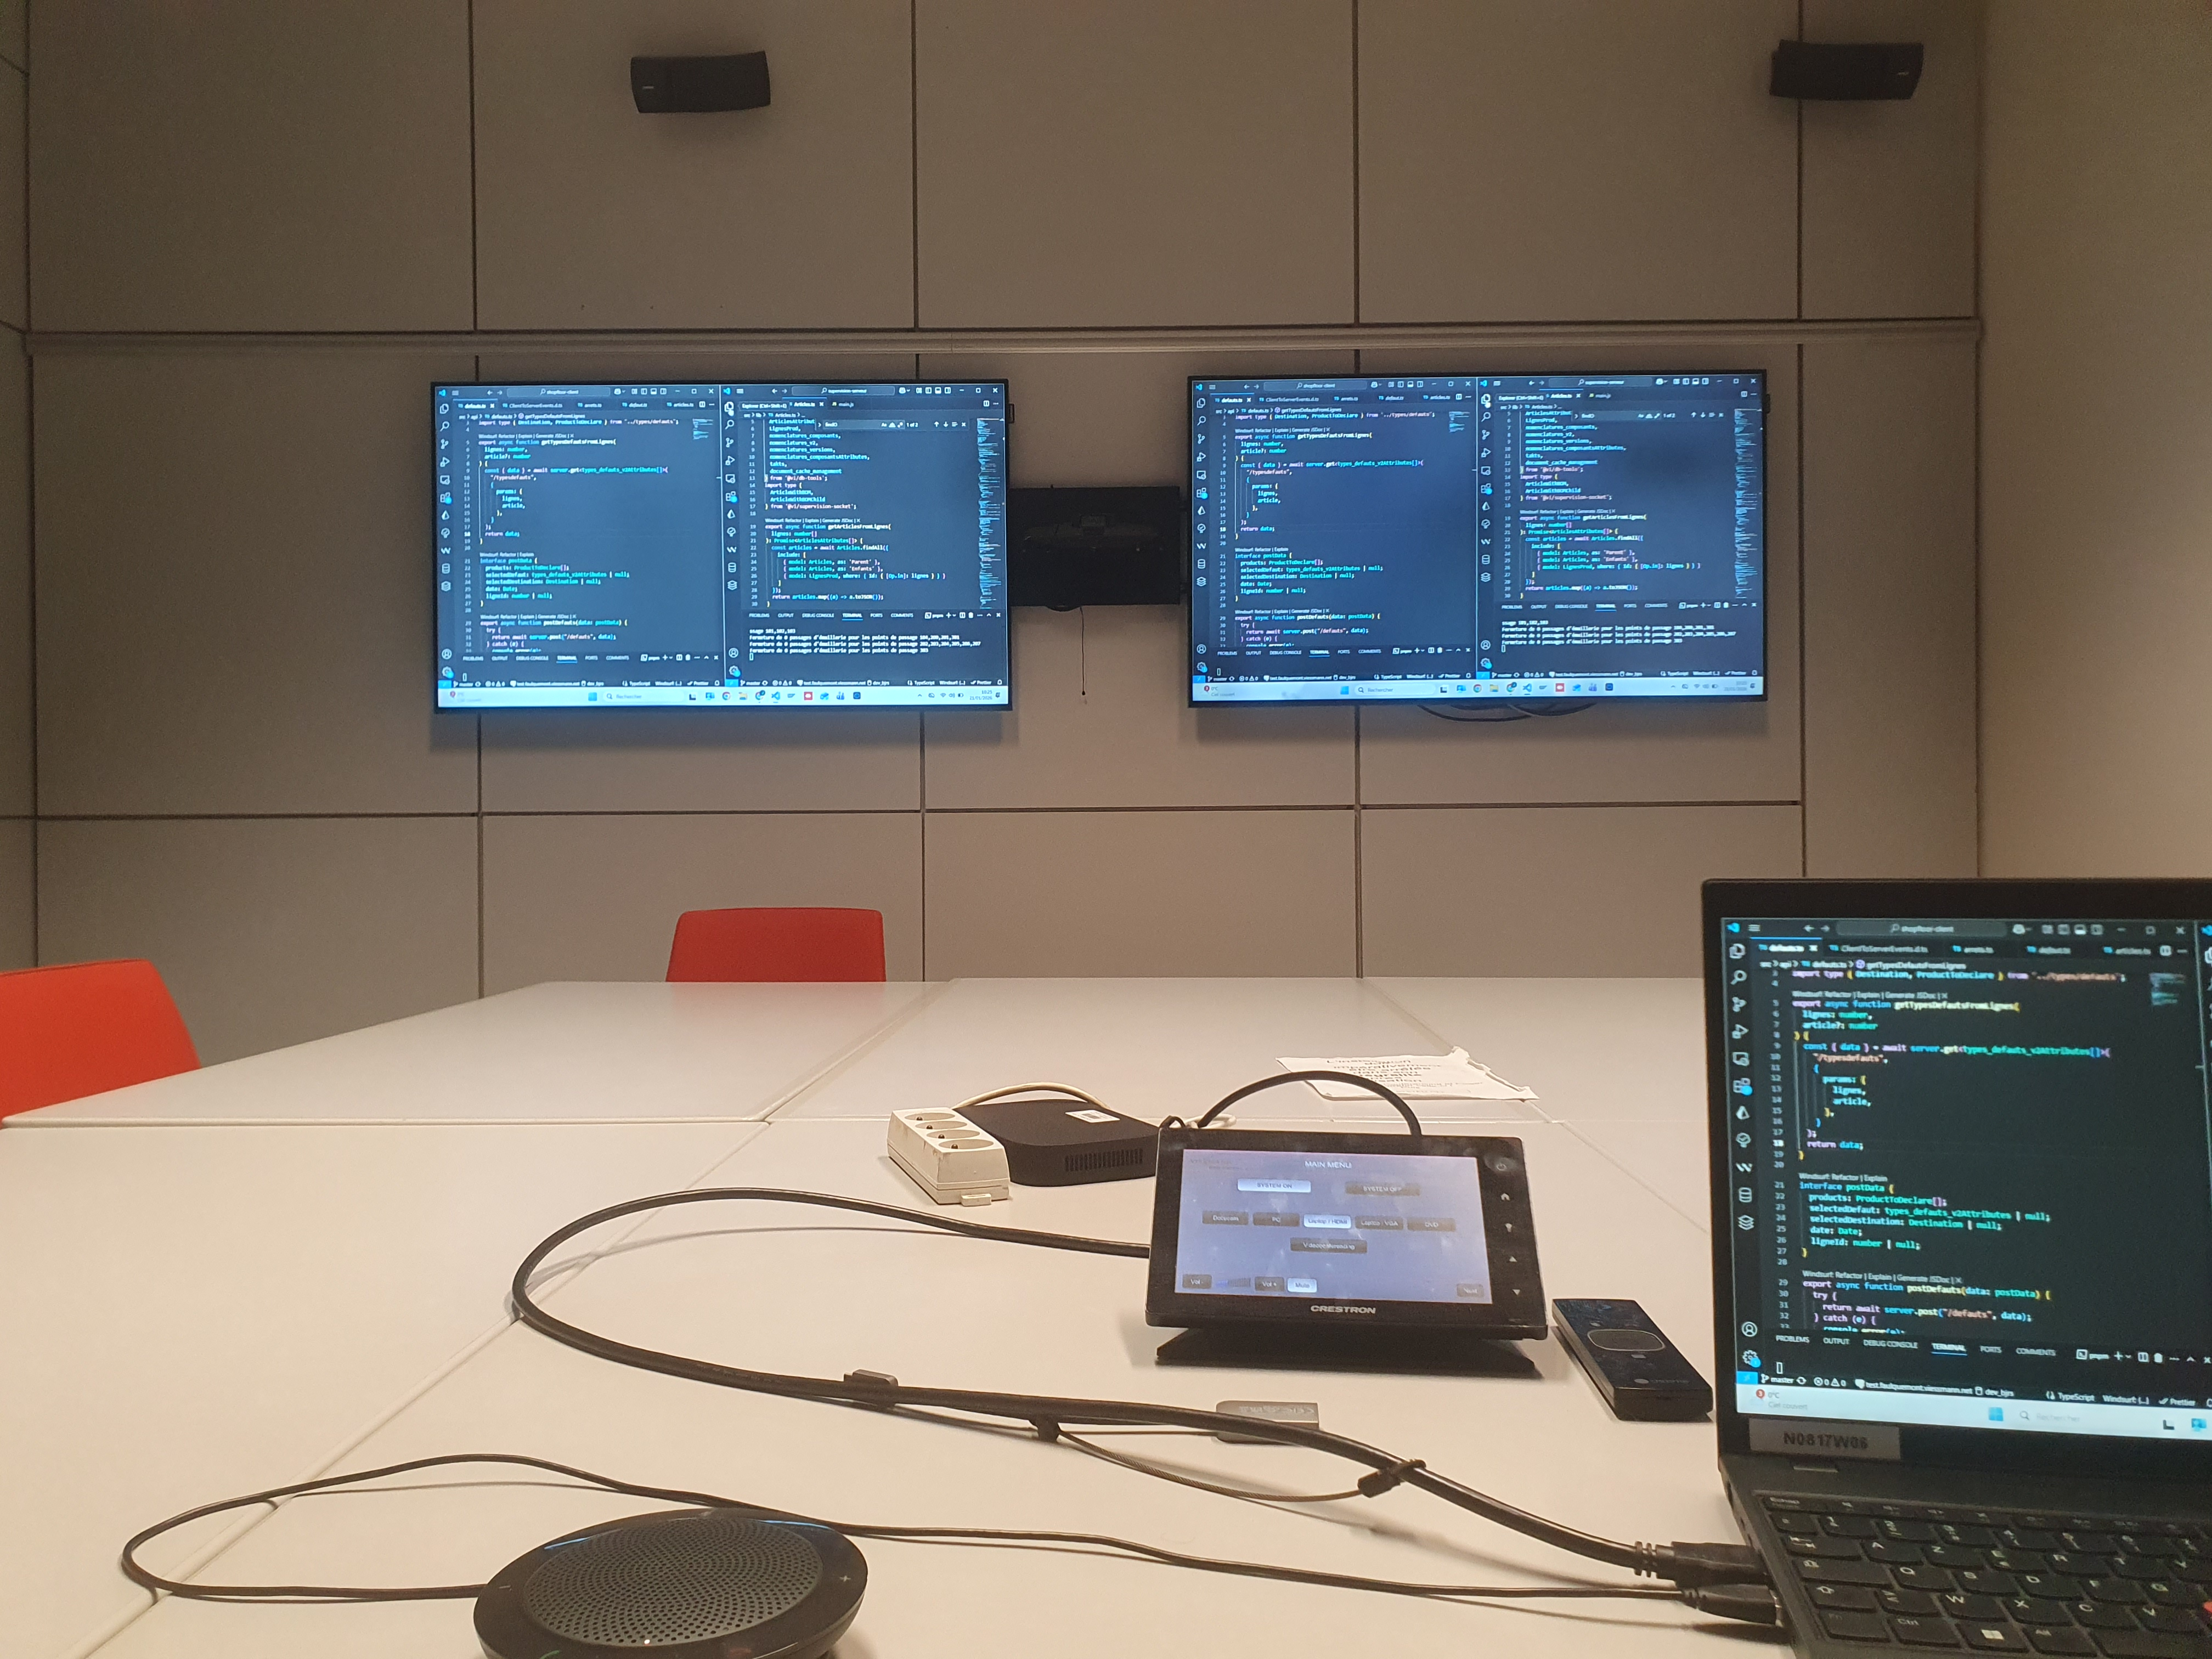
\includegraphics[width=0.8\textwidth]{figures/reunion_teams}
    \caption{Salle de réunion du Département Digitalisation, utilisée pour les visioconférences Teams}
    \label{fig:reunion-teams}
\end{figure}

La gestion des tâches au sein du département s'appuie sur Asana,
un outil de gestion de projet collaboratif en ligne. Chaque mission est
découpée en tâches individuelles, assignées à un responsable et associées
à une date d'échéance. Cet outil m'a permis de structurer mon travail au
quotidien : visualiser les priorités, suivre l'avancement de mes missions et
rendre compte de mes contributions de manière transparente à mon maître
d'apprentissage.

\cleardoublepage

\chapter{Présentation de deux missions significatives}

\section{Introduction des missions}

J'ai mené plusieurs missions au cours de cette première année d'apprentissage. 
Plutôt qu'une énumération exhaustive, j'ai choisi d'en présenter deux en 
détail, car elles me paraissent les plus représentatives à la fois de mon 
évolution sur l'année et de la diversité des compétences mobilisées.

La première mission, étant la mise en place d'un système d'appairage 
d'équipements via \gls{WebSocket}, m'a permis d'aborder pour la première fois 
les architectures temps réel et la gestion des états de connexion. 
Elle m'a fait travailler sur la communication en temps réel entre 
plusieurs appareils, un aspect du développement très utile pour n'importe quel type d'application.

La seconde mission, étant la gestion des lignes de production avec planification 
automatisée, est une fonctionnalité plus large. Elle m'a confronté à la 
modélisation métier, à l'intégration dans un code existant et à 
l'automatisation via des tâches planifiées. Pensée avant tout pour répondre 
à un besoin concret des utilisateurs, elle m'a fait suivre une fonctionnalité 
sur tout son cycle : comprendre le besoin, le traduire en quelque chose 
d'utilisable, puis le livrer accompagné de sa documentation.
Ces deux missions se complètent : l'une plus technique, l'autre plus 
proche du besoin des utilisateurs. Ensemble, elles donnent une bonne 
image du travail réalisé sur l'année.

\section{Mission 1 : Système de pairing d'équipements pour l'application Shopfloor}

\subsection{Contexte et enjeux}
L'application Shopfloor, développée en interne, est un outil global de 
gestion de la production. Elle permet notamment de planifier les postes 
de travail sur les lignes, de déclarer quotidiennement les pièces 
produites (bonnes, mauvaises, rebuts, réparées etc...), et de suivre les statistiques de 
production via des tableaux de bord dédiés. Elle intègre également 
plusieurs bibliothèques de référence ainsi que d'autres fonctionnalités de 
recherches et de déclarations.

Ainsi, elle est utilisée quotidiennement 
sur les lignes de production pour suivre l'activité et diffuser des 
informations en temps réel. Elle est consultée depuis des équipements variés : 
postes utilisateurs classiques, mais aussi téléviseurs affichant des \gls{andons}, 
tablettes utilisées par les opérateurs, etc.

Jusqu'alors, connecter un nouvel équipement n'était pas intégré dans l'application Shopfloor. 
La connexion devait s'effectuer à partir d'un portail de connexion interne. Ce qui posait plusieurs 
problèmes : friction pour les utilisateurs, risque de mauvaise manipulation 
sur des équipements partagés.

L'objectif était de concevoir un système de \textit{pairing} sécurisé 
permettant d'associer durablement un équipement à l'application, sans saisie 
de mot de passe, et avec reconnexion automatique au démarrage.

\subsection{Objectif et livrables}
\begin{itemize}
    \item Un mécanisme d'appairage par code court (4 caractères) ou QR code, 
    initié depuis l'équipement à connecter et validé depuis un poste 
    utilisateur déjà authentifié
    \item Une persistance du couplage, pour que l'équipement se reconnecte 
    automatiquement à chaque redémarrage
    \item Un mode d'affichage dédié aux équipements (interface adaptée)
    \item Une fonction de déconnexion accessible à la fois pour les 
    utilisateurs et les équipements
    \item Un article SharePoint à destination des utilisateurs finaux, 
    documentant la nouvelle fonctionnalité (voir Annexe~\ref{annexe:sharepoint-pairing})
\end{itemize}

\subsection{Démarche et outils mobilisés}
L'application est développée avec Express et \gls{Sequelize}
côté serveur, et \gls{Quasar} côté client. Le besoin de communication
temps réel m'a amené à utiliser le protocole \gls{WebSocket} : contrairement au HTTP 
traditionnel, il maintient une connexion persistante et bidirectionnelle 
entre le serveur et le client, ce qui permet au serveur d'envoyer 
instantanément un événement de validation à l'équipement en cours 
d'appairage.

    \begin{figure}[H]
        \centering
        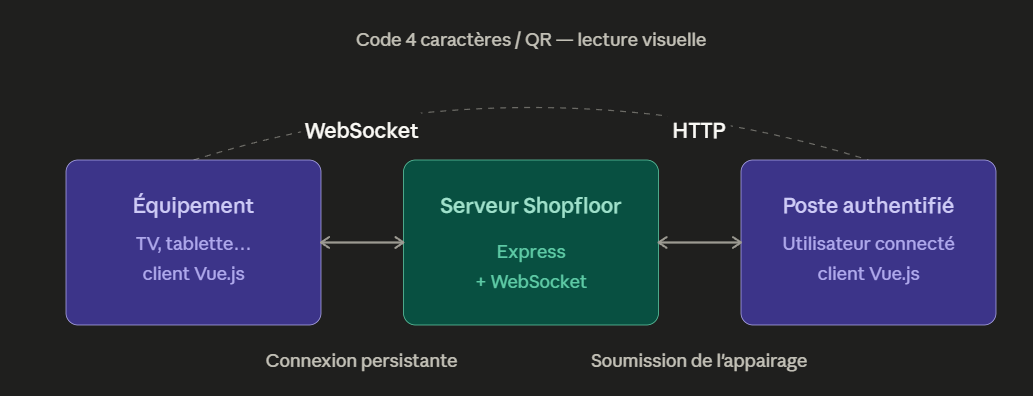
\includegraphics[width=0.7\textwidth]{figures/archi}
        \caption{Architecture de communication temps réel lors de l'appairage}
        \label{fig:archi-websocket}
    \end{figure}

Le flux d'appairage fonctionne ainsi :
\begin{enumerate}
    \item L'équipement à connecter ouvre la page de login et clique sur 
    « Lier un équipement ». Un code à 4 caractères et un QR code 
    équivalent sont générés, valables 5 minutes. 
    \begin{figure}[H]
        \centering
        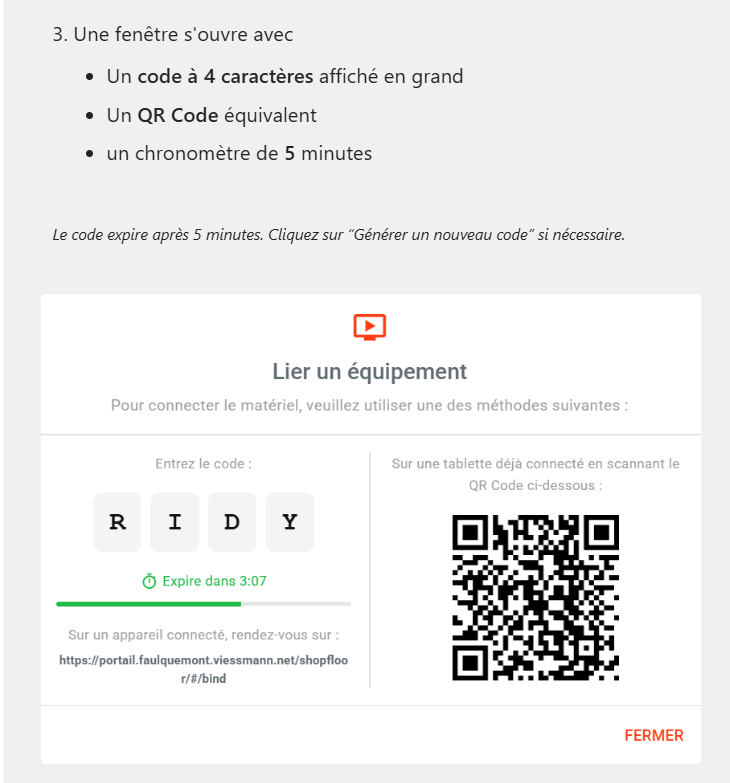
\includegraphics[width=0.7\textwidth]{figures/annexe1}
        \caption{Fenêtre de génération du code d'appairage}
        \label{fig:pairing-code}
    \end{figure}
    \item Sur un poste déjà authentifié, l'utilisateur scanne le QR code 
    ou saisit le code manuellement, sélectionne le service de rattachement auquel il est associé 
    et nomme l'équipement. (voir Annexe~\ref{annexe:sharepoint-pairing2})
    \item Côté serveur, l'association est validée et un token unique est 
    envoyé à l'équipement via \gls{WebSocket}. L'équipement est alors redirigé 
    vers l'accueil en mode équipement.
\end{enumerate}

La persistance du couplage repose sur deux mécanismes complémentaires :
\begin{itemize}
    \item Un \textbf{token d'authentification} unique, stocké côté équipement 
    et utilisé pour identifier toutes les communications \gls{WebSocket} ultérieures
    \item Une \textbf{reconnexion automatique basée sur l'adresse IP} de 
    l'équipement, qui permet de rétablir la session sans intervention humaine 
    après une coupure réseau ou un redémarrage.
\end{itemize}

\subsection{Difficultés rencontrées}
La principale difficulté de cette mission a été ma prise en main du 
protocole \gls{WebSocket}, que je n'avais jamais réellement utilisé jusque-là. 
Mon expérience du développement web reposait essentiellement sur le modèle 
requête-réponse classique de HTTP, et le passage à une communication 
bidirectionnelle persistante a nécessité un temps d'appropriation.

J'ai dû me familiariser avec plusieurs notions nouvelles : la gestion du 
cycle de vie d'une connexion (ouverture, maintien, fermeture), la 
distinction entre événements émis et événements reçus, et le fait que le 
serveur peut pousser une information vers le client sans que celui-ci l'ait 
demandée. Cette logique événementielle change la manière de structurer le 
code, aussi bien côté serveur que côté client.

Pour monter en compétence, je me suis appuyé sur la documentation officielle 
ainsi que sur des échanges avec mon maître d'apprentissage. J'ai également 
commencé par un prototype minimal pour valider mes hypothèses avant 
d'intégrer la logique dans l'application Shopfloor.

Un problème côté réseau subsiste néanmoins : au redémarrage des équipements, 
le serveur DHCP leur attribue parfois une adresse IP différente de celle 
enregistrée lors de l'appairage. Or, comme la reconnexion automatique 
s'appuie sur l'IP pour identifier l'équipement, ce changement empêche le 
système de rétablir la session sans nouvelle intervention.

\subsection{Résultats}
Le système de pairing est aujourd'hui déployé en production et utilisé par 
différents services dans l'usine. La 
documentation utilisateur diffusée via SharePoint (voir Annexe~\ref{annexe:sharepoint-pairing}) a permis une prise en main 
autonome par les équipes, sans formation dédiée.

\subsection{Apport personnel}
Cette mission m'a permis de découvrir en profondeur le protocole \gls{WebSocket} 
et les architectures temps réel, non abordés dans mon cursus jusqu'ici. 
Elle m'a également confronté aux contraintes spécifiques de l'environnement 
industriel, où la fiabilité prime sur les fonctionnalités, et m'a sensibilisé 
à l'importance de la documentation utilisateur dans le cycle de livraison 
d'une fonctionnalité.


\section{Mission 2 : Gestion des lignes de production et planification automatisée}

\subsection{Contexte et enjeux}
L'application Shopfloor intègre un planificateur de postes utilisé par les 
\textit{team leaders} et les \gls{IE} pour organiser le 
travail sur les lignes de production. Alors, la planification 
hebdomadaire était entièrement manuelle : chaque semaine, les responsables 
devaient recréer les postes de chaque ligne, ce qui représentait une charge 
de travail répétitive et une source d'erreurs.

L'observation des pratiques a fait émerger un constat : la majorité des 
lignes suivent un schéma hebdomadaire stable (mêmes équipes, mêmes 
modèles de postes d'une semaine à l'autre). Il devenait donc pertinent 
d'introduire la notion de \textbf{semaine type} : un modèle de semaine 
configurable pour chaque ligne, que l'on pourrait appliquer en un clic ou 
même de manière entièrement automatique.

La mission consistait à concevoir l'ensemble du dispositif : un référentiel 
des lignes de production, une fiche détaillée par ligne, un éditeur de 
semaine type, l'intégration de nouvelles actions dans le planificateur 
existant, et enfin l'automatisation hebdomadaire de l'application des 
semaines types.

\subsection{Objectif et livrables}
\begin{itemize}
    \item Une \textbf{bibliothèque des lignes de production} accessible 
    depuis le menu de l'application, listant les lignes actives regroupées 
    par étape de flux, avec recherche et indicateur de configuration.
    \item Une \textbf{fiche détail} pour chaque ligne, organisée en trois 
    onglets : informations générales, défauts associés, et semaine type
    \item Un \textbf{formulaire de modification} couvrant l'ensemble des 
    champs configurables d'une ligne (identité, configuration 
    fonctionnelle, relations avec d'autres lignes).
    \item De nouvelles \textbf{actions dans le planificateur} : appliquer 
    manuellement une semaine type, ou enregistrer la semaine courante 
    comme nouveau modèle.
    \item Un \textbf{job d'automatisation hebdomadaire} appliquant la 
    semaine type sur toutes les lignes dont la semaine suivante est vide.
    \item Une \textbf{gestion des droits} en fonction du rôle 
    (opérateur, \textit{team leader}, responsable de secteur, \gls{IE}).
    \item Un \textbf{article de documentation} à destination des 
    utilisateurs, publié sur SharePoint.
\end{itemize}

\subsection{Démarche et outils mobilisés}
Pour rappel, l'application est développée avec Express et \gls{Sequelize}
côté serveur, et \gls{Quasar} côté client. L'automatisation des
actions planifiées s'appuie sur la librairie node-schedule, qui permet de définir 
des jobs récurrents selon une syntaxe \textit{\gls{cron}}.

Le travail s'est articulé autour de plusieurs sous-ensembles :

Avant le développement, j'ai réfléchi à la modélisation de la semaine 
type en base de données : comment représenter le lien entre une ligne, 
les jours de la semaine, et les modèles de postes applicables, tout en 
restant suffisamment souple pour autoriser plusieurs modèles par jour.

J'ai finalement identifié la bonne relation à modéliser, ce qui m'a permis
de ramener l'ensemble à une seule table d'association et d'obtenir un
schéma de base de données plus simple et plus efficace.

\begin{figure}[H]
    \centering
    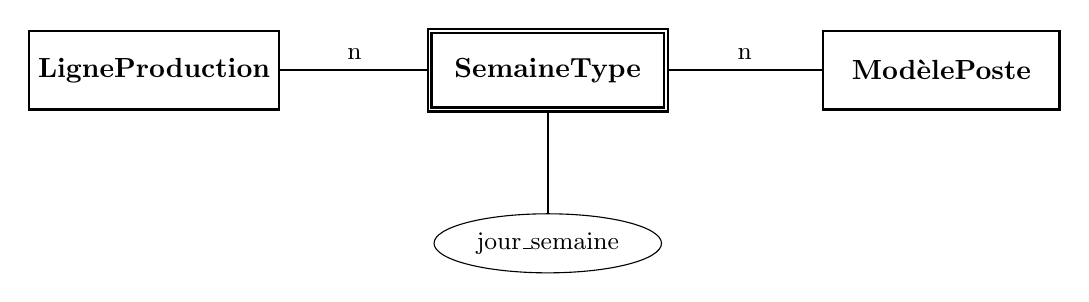
\begin{tikzpicture}[
        entity/.style={rectangle, draw=black, thick, minimum width=3cm, minimum height=1cm, align=center},
        assocent/.style={rectangle, draw=black, thick, double, minimum width=3cm, minimum height=1cm, align=center},
        attribute/.style={ellipse, draw=black, minimum width=2.2cm, minimum height=0.75cm, align=center, font=\small},
        line/.style={thick},
    ]
        \node[entity]   (ligne)   at (0, 0)    {\textbf{LigneProduction}};
        \node[assocent] (semaine) at (5, 0)    {\textbf{SemaineType}};
        \node[entity]   (modele)  at (10, 0)   {\textbf{ModèlePoste}};
        \node[attribute](jour)    at (5, -2.2) {jour\_semaine};

        \draw[line] (ligne)   -- node[above, font=\small]{n} node[below, font=\small]{} (semaine);
        \draw[line] (semaine) -- node[above, font=\small]{n} node[below, font=\small]{} (modele);
        \draw[line] (semaine) -- (jour);
    \end{tikzpicture}
    \caption{Schéma Entité-Association simplifié de la semaine type}
    \label{fig:ea-semaine-type}
\end{figure}

La table \textit{SemaineType} constitue l'unique lien entre une ligne de
production, un jour de la semaine et un modèle de poste. Les cardinalités \textbf{n} des deux côtés reflètent une relation
\textbf{n-n} : une même ligne de production peut apparaître plusieurs fois
dans la table, car un même jour peut concentrer plusieurs modèles de postes
sur cette ligne (un enregistrement par couple jour/modèle). De même, un même
modèle de poste peut être utilisé sur plusieurs lignes ou plusieurs jours.
Cette relation se traduit, en base de données, par une table avec deux clés
étrangères (\textit{id\_ligne}, \textit{id\_modele}) et un attribut
\textit{jour\_semaine}, dont la combinaison identifie chaque entrée.

La bibliothèque et la fiche détail ont été conçues pour offrir une 
lecture rapide aux responsables : regroupement par étape de flux, 
indicateur visuel du nombre de lignes configurées, accès en 
un clic à la fiche détail. L'interface adapte les fonctionnalités 
disponibles selon le rôle de l'utilisateur connecté.


L'ajout des actions « Appliquer la semaine type » et « Enregistrer 
comme semaine type » a nécessité de me plonger dans le code existant 
du planificateur pour l'enrichir sans rupture pour les utilisateurs 
actuels. Une fenêtre de confirmation permet à l'utilisateur de choisir 
l'équipe associée à chaque modèle de poste lors de l'application.


Un job node-schedule s'exécute tous les dimanches à 22h. Il parcourt 
les lignes de production ayant une semaine type configurée, vérifie 
que la semaine suivante est vide, et applique automatiquement le 
modèle si la semaine est en effet bien vide. Ce mécanisme libère les responsables d'une 
tâche purement répétitive et garantit qu'aucune ligne ne se retrouve 
sans planning par oubli.

\subsection{Difficultés rencontrées}
La principale difficulté de cette mission a été la persistance du 
job planifié après un redémarrage du serveur. N'ayant jamais utilisé la 
librairie \text{node-schedule}, je ne savais pas comment se comporterait 
le système au redémarrage : le \gls{cron} resterait-il enregistré, 
ou disparaîtrait-il avec le processus ?

J'ai rapidement compris qu'un job \text{node-schedule} vit en mémoire et 
ne survit pas à un redémarrage du \textit{backend}. J'ai donc mis en place 
un enregistrement automatique du job au démarrage du serveur : à chaque 
lancement, le cron est réinitialisé pour s'exécuter tous les dimanches à 
22h, et c'est lui qui, à ce moment-là, va lire la base de données et 
remplir les postes vides pour les lignes ayant une semaine type configurée.

Une seconde difficulté concernait la diffusion en temps réel des 
postes nouvellement créés aux utilisateurs déjà connectés à l'application. 
Lorsqu'un \gls{cron} déclenchait la création de postes le dimanche soir, ou 
lorsqu'un \textit{team leader} appliquait manuellement une semaine type, 
il fallait que les autres utilisateurs visualisent immédiatement les 
changements sans avoir à rafraîchir leur page. Je me suis appuyé sur une fonction utilisant
\gls{WebSocket}, déjà utilisé dans l'application, pour émettre 
les nouveaux postes à l'ensemble des clients connectés.

\subsection{Résultats}
La fonctionnalité est aujourd'hui utilisée par certaines lignes de production et fait gagner un temps significatif aux responsables 
chaque semaine. L'application automatique du dimanche soir a éliminé les 
oublis de planification constatés auparavant le lundi matin. 
La documentation associée, diffusée sur SharePoint, a permis aux 
utilisateurs de découvrir les nouvelles fonctionnalités en autonomie.

\begin{figure}[H]
        \centering
        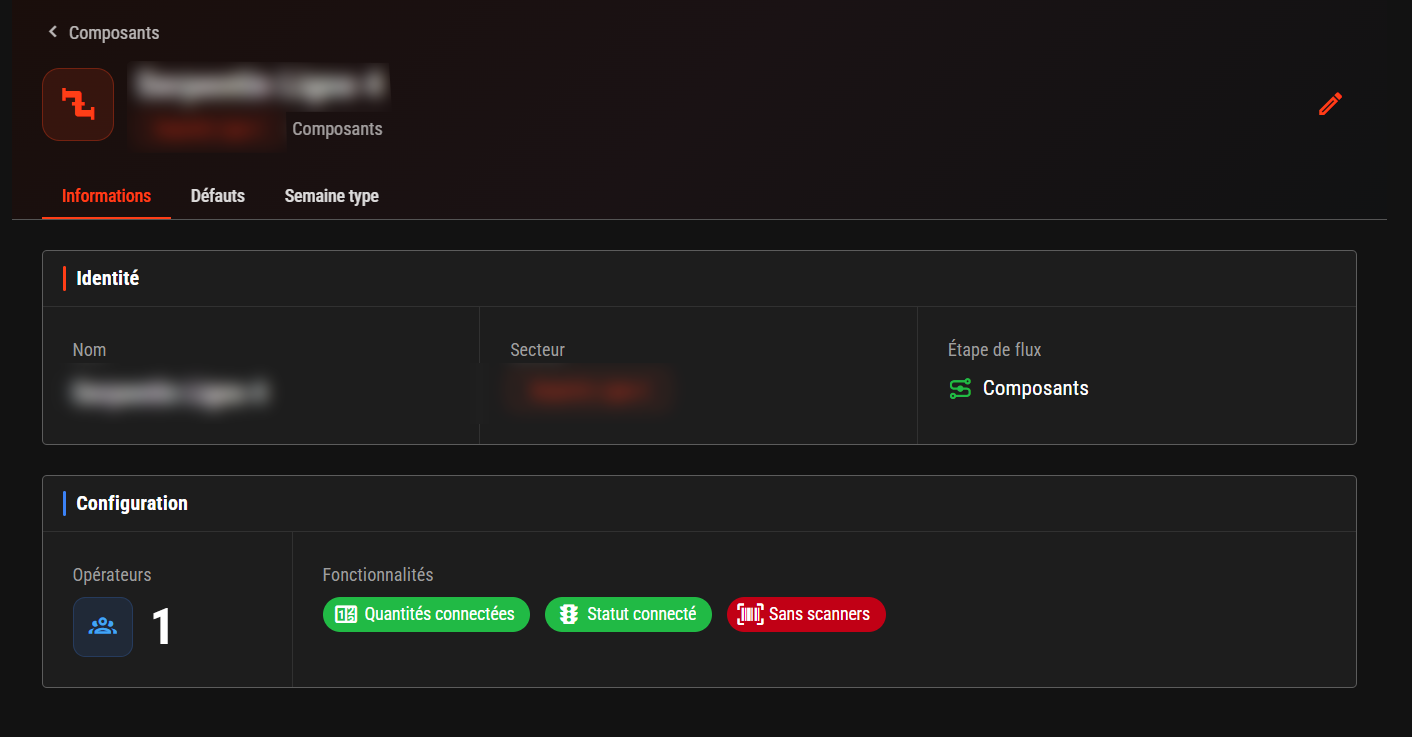
\includegraphics[width=1\textwidth]{figures/details}
        \caption{Page de détail d'une ligne de production }
        \label{fig:details-ligne}
    \end{figure}
\subsection{Apport personnel}
Cette mission, plus longue et plus large que la précédente, m'a 
confronté à la conception d'une fonctionnalité dans son intégralité : 
analyse du besoin métier, modélisation des données, conception 
d'interface, intégration dans une application existante, et 
automatisation. Elle m'a permis de découvrir les systèmes de tâches 
planifiées et de mesurer l'impact 
concret qu'une automatisation bien pensée peut avoir sur le quotidien 
des équipes de production.

\chapter{Compétences acquises et analyse réflexive}

Au-delà des livrables eux-mêmes, cette première année d'apprentissage m'a 
permis de développer plusieurs compétences que je souhaite mettre en lumière 
dans ce chapitre, qu'elles soient techniques, transversales, ou liées au 
rapport entre théorie et pratique.

\section{Compétences techniques}

J'ai approfondi mes connaissances des frameworks \textbf{Express},
\textbf{\gls{Quasar}} et \textbf{\gls{Sequelize}}, en les pratiquant dans le
contexte d'une application réellement utilisée. Travailler dans un code 
existant, parfois ancien, m'a appris à lire avant d'écrire, à comprendre les 
décisions prises avant moi et à intégrer mes propres ajouts sans rupture et/ou effets secondaires ou non voulus.

Plusieurs technologies nouvelles se sont également ajoutées à mon bagage :
\begin{itemize}
    \item Le protocole \gls{WebSocket} et plus généralement les 
    architectures temps réel, avec leurs spécificités
    \item La planification de tâches automatisées avec node-schedule, 
    et la réflexion qui l'accompagne sur la robustesse des jobs récurrents.
    \item La modélisation de données métier, en réfléchissant à des schémas 
    suffisamment souples pour absorber l'évolution des besoins.
\end{itemize}

\section{Compétences transversales}

% \paragraph{Communication technique et vulgarisation}
La rédaction d'articles SharePoint à destination des utilisateurs finaux 
m'a poussé à reformuler des fonctionnalités techniques en langage clair et 
illustré, accessible à des opérateurs ou des responsables qui n'ont pas forcément de 
culture informatique. Cet exercice m'a appris à me décentrer du point de vue 
du développeur et à structurer une explication autour de l'usage plutôt 
que de l'implémentation.

La montée en autonomie au fil de l'année m'a amené à mieux organiser mon 
travail : prioriser les tâches, estimer la charge d'une fonctionnalité, 
savoir quand demander de l'aide et quand chercher seul.

% \paragraph{Compréhension des besoins métier}
Les échanges réguliers avec mon maître d'apprentissage m'ont fait prendre 
conscience du décalage qui peut exister entre un besoin formulé et le besoin 
réel souhaité. Apprendre à poser les bonnes questions avant de coder est 
un apport important de cette année.

\section{Lien entre la formation et la pratique}

Certaines notions vues en formation se sont révélées utiles sur le terrain : 
des principes généraux d'architecture 
logicielle, par exemple, m'ont aidé à comprendre l'organisation des 
applications sur lesquelles j'ai travaillé.

En revanche, je dois être honnête sur un point : les enseignements de 
développement web suivis à l'école ne suffisaient pas, à eux seuls, à mener 
à bien les missions qui m'ont été confiées. Les frameworks et technologies 
utilisés en entreprise (Vue.js, Express, \gls{WebSocket}, et plus généralement 
l'écosystème JavaScript moderne) n'étaient que peu ou pas abordés dans le 
cursus. J'ai pu compenser cet écart grâce aux connaissances que j'avais 
déjà acquises par moi-même avant l'apprentissage, et surtout grâce à un travail 
de formation autonome continu : lecture de documentation, expérimentation, 
et appui sur les retours de mon maître d'apprentissage.

Cette situation, loin d'être un point négatif, m'a fait prendre conscience 
d'une compétence essentielle du métier d'ingénieur : la capacité à 
apprendre seul et à monter rapidement en compétence sur une technologie 
inconnue. Une formation ne peut pas couvrir l'intégralité des outils 
employés en entreprise, et savoir combler soi-même cet écart est sans doute 
aussi important que les connaissances elles-mêmes. L'apprentissage m'a ainsi 
apporté ce que les cours ne pouvaient pas offrir : la conduite d'un projet, le travail dans un code existant, et la gestion des 
contraintes réelles de production.

\section{Analyse réflexive}

\subsubsection{Ce qui a bien fonctionné}
Mon intégration dans l'équipe et la prise en main de l'application se sont 
faites rapidement. La rigueur acquise en formation, notamment dans la 
structuration du code, m'a permis de produire un travail 
exploitable dès les premiers mois.

\subsubsection{Ce que je referais différemment}
Avec le recul, je consacrerais davantage de temps à la phase de conception 
en amont de certaines missions. À plusieurs reprises, j'ai commencé à coder 
trop tôt pour livrer plus vite et j'ai dû revenir en arrière sur des choix de modélisation. La 
mission de gestion des lignes de production m'a particulièrement fait 
prendre conscience de cet enjeu.

\subsubsection{Points encore à travailler}
Plusieurs axes d'amélioration restent à explorer. Je souhaiterais d'abord 
développer la documentation technique de mon code, que je néglige 
parfois au profit de l'implémentation, alors qu'elle est essentielle à la 
maintenabilité d'un projet sur le long terme. Ensuite, je voudrais 
renforcer ma maîtrise des bonnes pratiques de conception, 
notamment autour des API RESTful, dont je n'ai pas toujours respecté les 
conventions par manque de méthode. Enfin, je gagnerais à instaurer une 
véritable veille technologique régulière, pour découvrir des 
outils, des approches et des patterns qui me feront progresser au-delà 
des seuls besoins de mes missions.

\cleardoublepage

\chapter{Bilan et perspectives}

\section{Bilan global de l'année}

Cette première année d'apprentissage a été à la hauteur de mes attentes. Elle 
m'a permis de confirmer mon attrait pour le développement logiciel en 
contexte industriel, où la technique alimente un objectif métier concret et 
mesurable. Les fonctionnalités que j'ai livré sont utilisées 
quotidiennement par les équipes de production, ce qui donne au travail un 
sens immédiat et motivant.

Sur le plan personnel, cette année m'a apporté une plus grande confiance 
dans ma capacité à prendre en charge une fonctionnalité dans son ensemble, 
de la compréhension du besoin jusqu'à la livraison et la documentation.

\section{Objectifs et axes de progression pour la deuxième année}

Pour la deuxième année d'apprentissage, je me fixe plusieurs objectifs, dont 
certains rejoignent directement les ambitions du Département Digitalisation.

Le département, dirigé par mon maître d'apprentissage, souhaite intégrer 
l'intelligence artificielle de manière réfléchie et progressive dans ses 
activités, puis plus largement au sein de Viessmann. Dans cette perspective, 
l'un des projets envisagés est le développement d'un agent IA 
interne, propre au département. Cet agent pourrait par exemple prendre la 
forme d'un assistant à destination des développeurs, facilitant leur travail 
au quotidien. Contribuer à ce projet constitue pour moi un axe de travail 
majeur pour l'année à venir : il me permettrait de découvrir un domaine en 
pleine évolution tout en répondant à un besoin concret de l'entreprise.

Cet objectif suppose un important travail de montée en compétence, car il 
s'agit pour moi d'un domaine entièrement nouveau. Je devrai me former aux 
concepts fondamentaux de l'IA appliquée : le fonctionnement des modèles de 
langage, le \textit{function calling} (qui permet à un agent d'exécuter 
des actions concrètes via des outils externes), les architectures d'agent, 
ainsi que les approches permettant à un agent de s'appuyer sur des sources 
de connaissances internes comme les \textit{embeddings} et \textit{RAG} 
(\textit{Retrieval-Augmented Generation}). Je m'intéresserai également au 
\textit{Model Context Protocol} (MCP), un standard récent permettant de 
connecter de manière unifiée un agent à différents outils et sources de 
données.

Cet objectif tombe à point nommé puisque la deuxième année de formation 
comporte justement plusieurs cours dédiés à l'intelligence artificielle. 
Je pourrai ainsi tirer parti de cette complémentarité directe entre les 
apports théoriques de l'école et les besoins concrets de l'entreprise, ce 
qui est l'un des grands intérêts de la formation en apprentissage.

À cela s'ajoutent plusieurs objectifs personnels :
\begin{itemize}
    \item \textbf{Mettre en place une veille technologique régulière} pour 
    découvrir de nouveaux outils, approches et bonnes pratiques au-delà des 
    besoins immédiats de mes missions.
    \item \textbf{Gagner en autonomie sur la conception} en amont des 
    développements, en m'impliquant davantage dès l'analyse du besoin
    \item \textbf{Approfondir ma compréhension du métier} de la production 
    industrielle, pour mieux anticiper les besoins des utilisateurs.
\end{itemize}

\cleardoublepage

\chapter{Conclusion}
\addcontentsline{toc}{chapter}{Conclusion}

Cette première année d'apprentissage chez Viessmann m'a permis de 
m'immerger dans un environnement industriel à forte composante numérique 
et de contribuer concrètement, à mon échelle, à la modernisation des 
outils internes du Département Digitalisation. Les deux missions 
présentées dans ce rapport ; le système d'appairage d'équipements et la 
gestion automatisée des lignes de production illustrent la diversité 
des compétences mobilisées sur l'année, des architectures temps réel à 
la modélisation métier, en passant par la planification de tâches et la 
documentation à destination des utilisateurs.

Au-delà des fonctionnalités livrées, cette année m'a apporté une vision 
plus mature du métier d'ingénieur logiciel : il ne s'agit pas seulement 
d'écrire du code, mais de comprendre un besoin, de concevoir une réponse 
adaptée et de la livrer accompagnée de tout ce qui permettra aux 
utilisateurs de s'en saisir. Elle m'a également confirmé l'importance, 
dans ce métier, de savoir monter en compétence en autonomie sur des 
technologies inconnues.

Les objectifs que je m'étais fixés en introduction me semblent 
globalement atteints, même si plusieurs axes resteront à explorer pour 
la deuxième année : renforcer la conception en amont des développements, 
instaurer une véritable veille technologique, et surtout contribuer au 
projet d'agent IA porté par le département. Ce dernier sujet 
ouvrira un champ entièrement nouveau pour moi, en lien direct avec les 
cours d'intelligence artificielle prévus dans ma deuxième année de 
formation. C'est dans cette perspective que j'aborde la suite de mon 
parcours en apprentissage, avec la motivation renouvelée que cette 
première année m'a apportée.

\cleardoublepage

\renewcommand{\tocbibname}{Bibliographie / Webographie}
\bibliographystyle{unsrt}
\nocite{*}
\bibliography{example} % See example.bib

\cleardoublepage


\printglossaries

\cleardoublepage
\renewcommand{\thesubsection}{\Roman{subsection}}

\appendix
\part*{Annexes}
\addcontentsline{toc}{part}{Annexes}

\chapter{Première Annexe}

\begin{figure}[h]
  \centering
  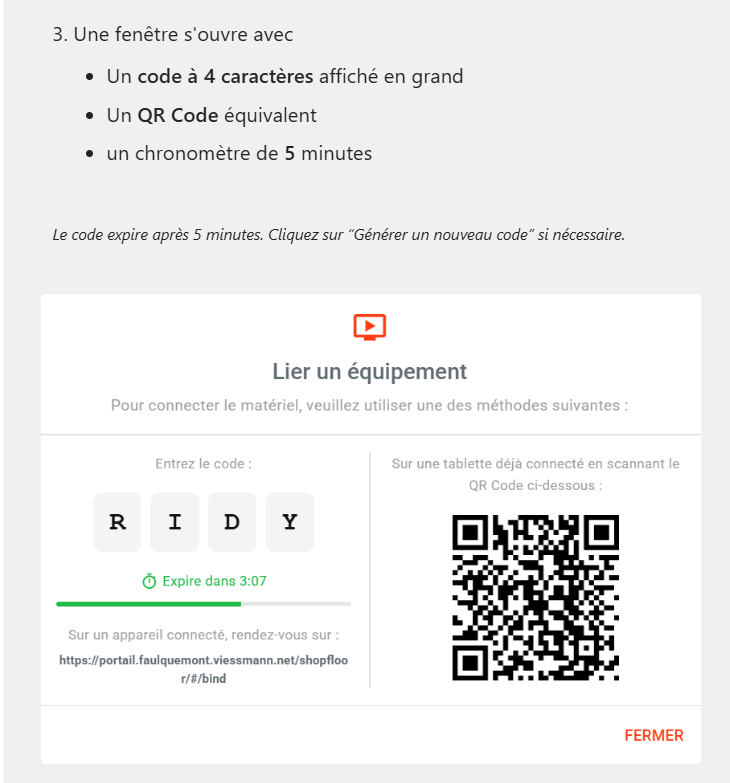
\includegraphics[width=0.9\textwidth]{figures/annexe1}
  \caption{Documentation utilsateur (1)}
  \label{annexe:sharepoint-pairing}
\end{figure}
\begin{figure}[h]
  \centering
  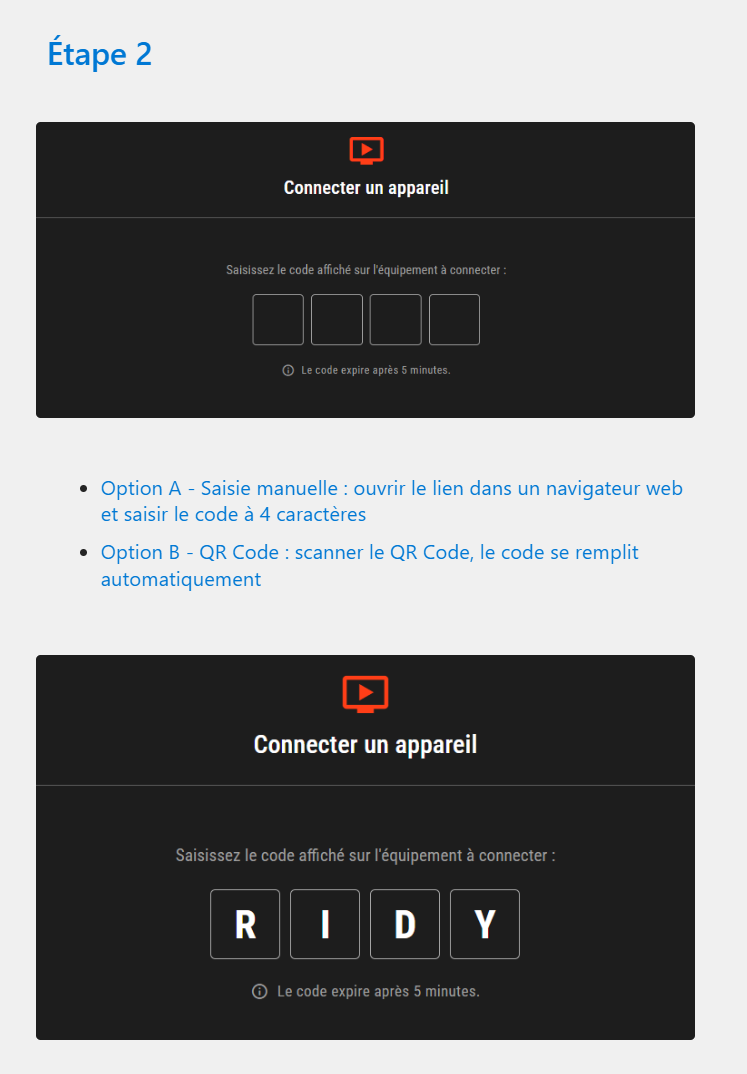
\includegraphics[width=0.9\textwidth]{figures/annexe2}
  \caption{Documentation utilisateur (2)}
  \label{annexe:sharepoint-pairing2}
\end{figure}
\begin{figure}[h]
  \centering
  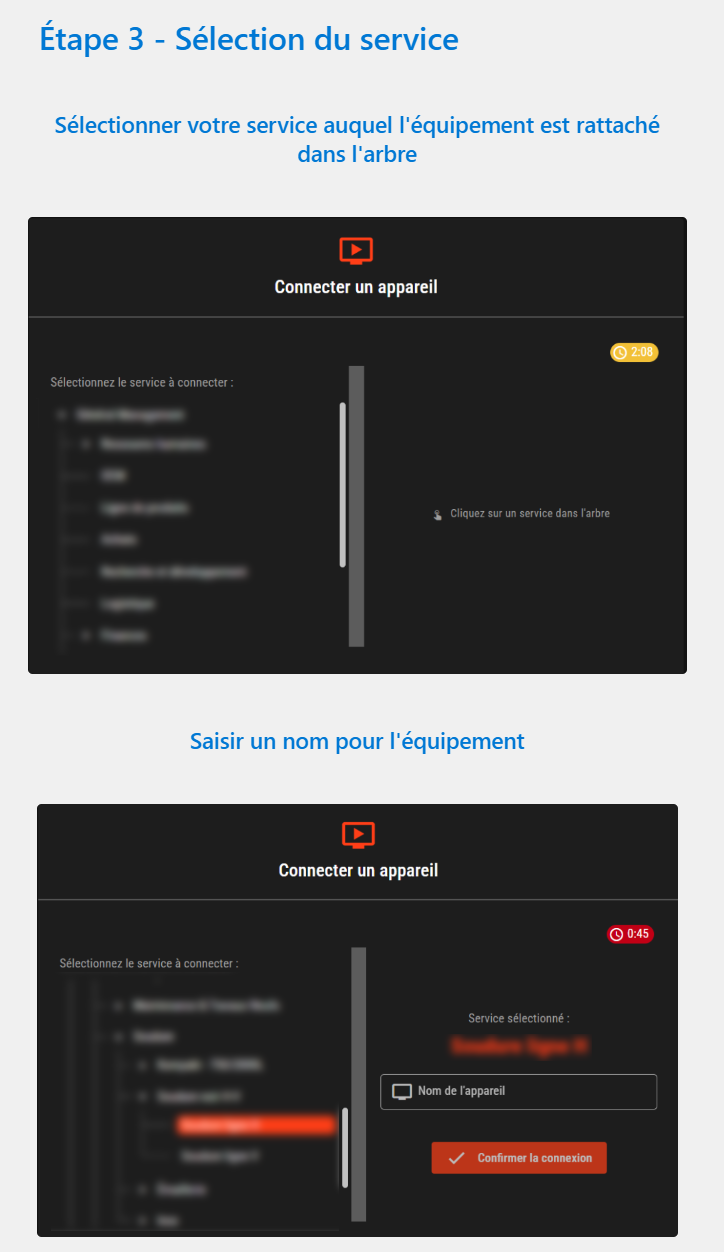
\includegraphics[width=0.9\textwidth]{figures/annexe3}
 \caption{Documentation utilisateur (3)}
\end{figure}

\chapter{Seconde Annexe}
\begin{figure}[h]
  \centering
  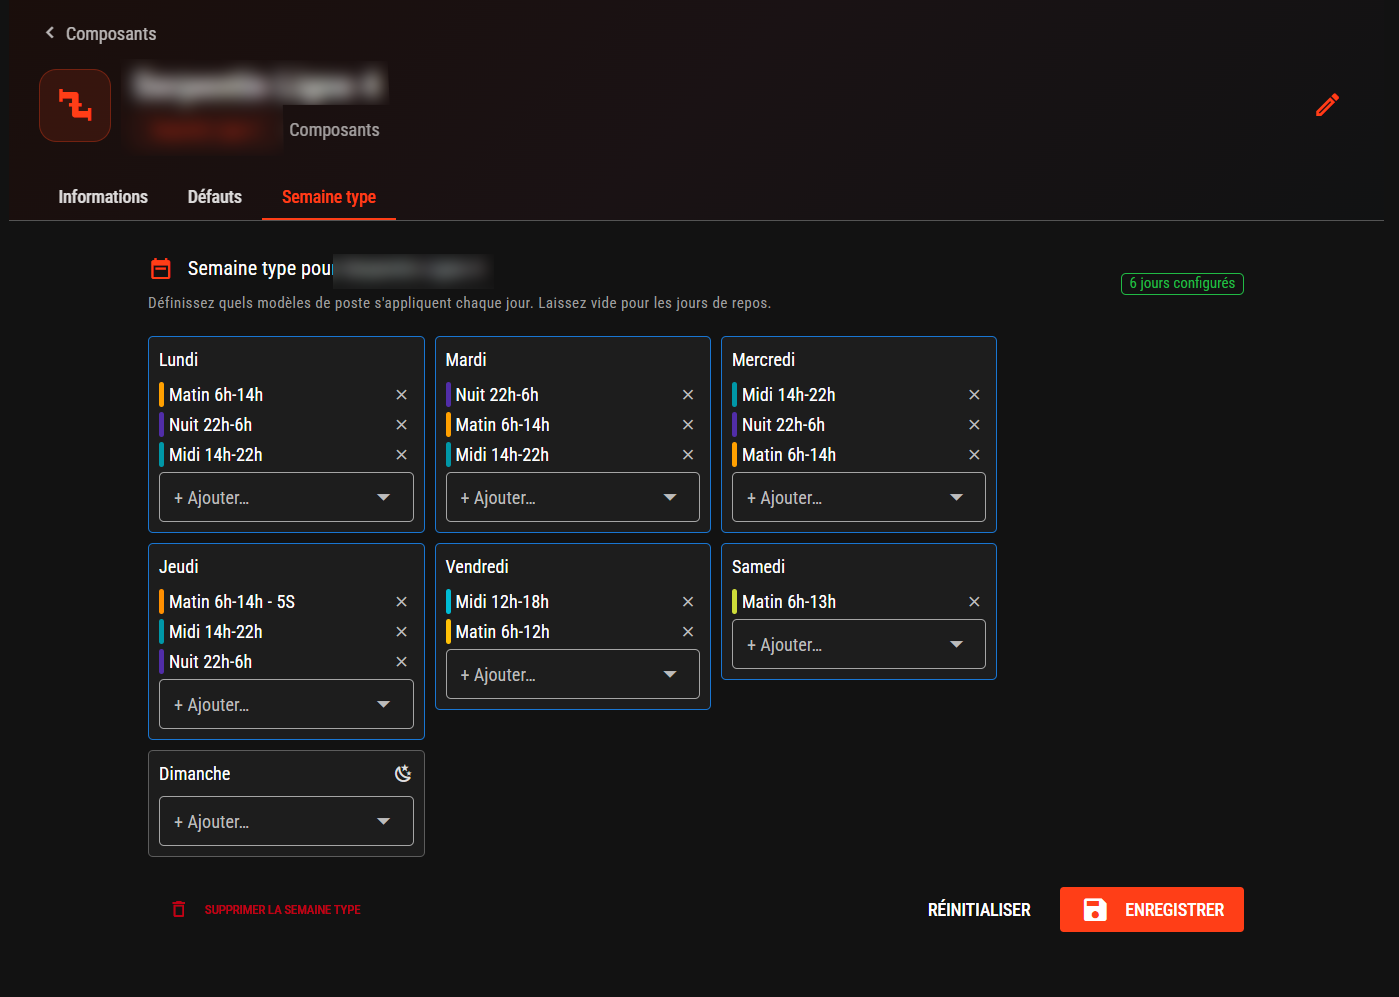
\includegraphics[width=0.9\textwidth]{figures/semaine}
  \caption{Page pour créer des semaines type de postes}
  \label{annexe:détails}
\end{figure}

\begin{figure}[h]
  \centering
  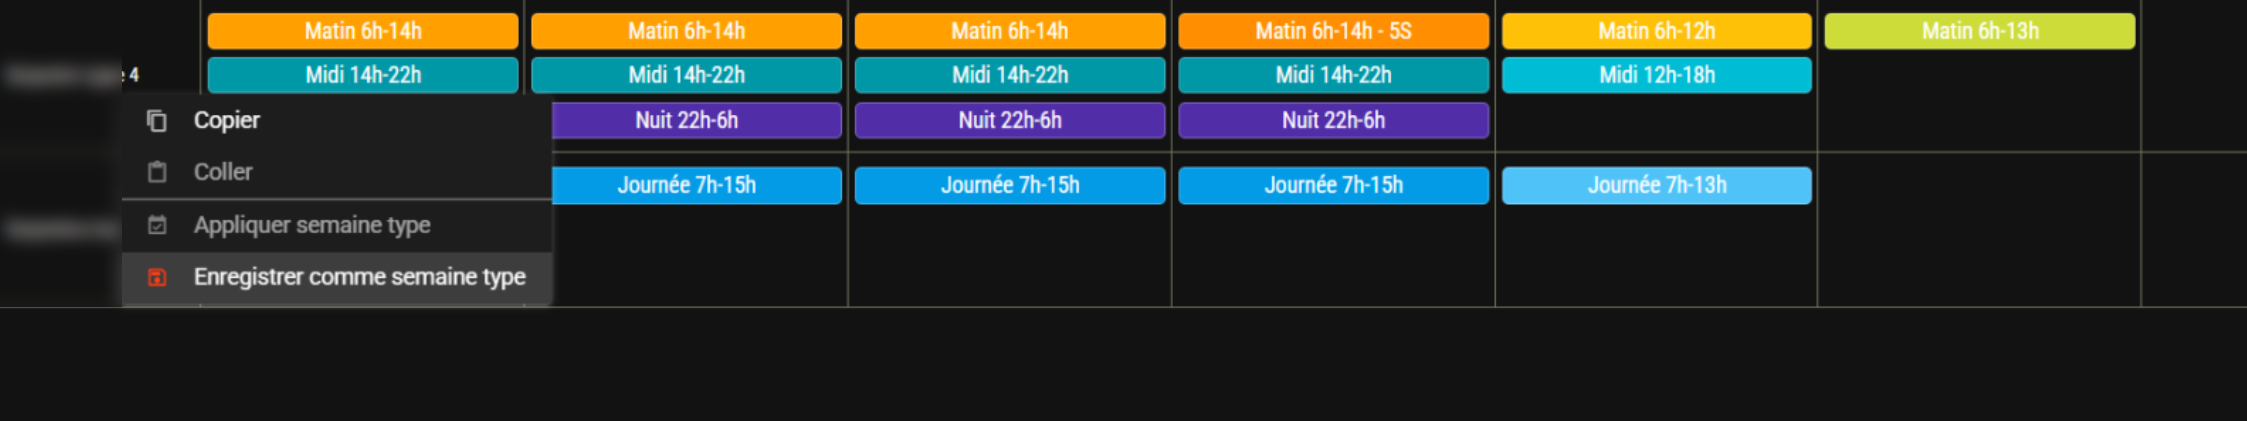
\includegraphics[width=0.9\textwidth]{figures/type}
  \caption{Nouvelles actions dans le planificateur de postes}
  \label{annexe:détails}
\end{figure}


\end{document}
